\PassOptionsToPackage{quiet}{xeCJK}
\documentclass[12pt, a4paper, twoside]{ctexbook}
\usepackage{amsmath,amsthm,amssymb,bm,graphicx,hyperref,mathrsfs,geometry,booktabs,makecell,mathcomp,esint,upgreek}
\usepackage{mwe,color,float,cleveref}
\usepackage{tabularx,multirow,array,caption}
\usepackage[T1]{fontenc}

\extrafloats{150}
\graphicspath{{Figures/}}
\hypersetup{colorlinks=true, linkcolor=black}
\geometry{left=2.0cm, top=2.0cm, bottom=2.0cm, right=2.0cm}

\title{{\Huge{\textbf{物理学及其工程应用笔记(只是第八单元且复刻版)}}}}
\author{在我电脑上显示不出来啊啊啊啊啊啊啊啊啊啊呜呜呜呜}
\date{\today}


\linespread{1.5}
\newCJKfontfamily\sonti{FandolSong-Bold}

\newtheorem{theorem}{定理}[section]
\newtheorem{definition}[theorem]{定义}
\newtheorem{lemma}[theorem]{引理}
\newtheorem{corollary}[theorem]{推论}
\newtheorem{example}[theorem]{例}
\newtheorem{proposition}[theorem]{命题}

\captionsetup{format=hang}
\DeclareCaptionLabelSeparator*{sspace}{\ \ }
\captionsetup[figure]{labelsep=sspace}
\captionsetup[table]{labelsep=sspace}
\DeclareCaptionFont{heiti}{\heiti}
\DeclareCaptionFont{5hao}{\zihao{5}}
\captionsetup{labelfont={heiti,5hao},textfont={heiti,5hao}}

\crefname{figure}{图}{图}
\crefname{table}{表}{表}
\crefname{equation}{式}{式}
\hypersetup{breaklinks,colorlinks}
\hypersetup{hidelinks,bookmarksnumbered=true,bookmarksopen=true,pdfstartview=Fit}

\everymath{\displaystyle}


\begin{document}


\pagestyle{plain}
	
	\newpage
    \tableofcontents
    \setcounter{page}{2}



\chapter*{热力学基础}
\addcontentsline{toc}{chapter}{热力学基础}


\renewcommand\thesection{\arabic {section}}
\section{名词解释}
\textbf{非平衡过程(非静态过程):}系统在整个过程中将经历一系列的非平衡态,这样的过程称为\textbf{非平衡过程(非静态过程)}

\textbf{准静态过程:}如果系统在过程进行中,每一个中间状态的变化进行得无限缓慢,使得任意时刻所经历的中间状态都无限地接近平衡态,则这样的过程称为\textbf{准静态过程}。准静态过程是理想化、抽象化的

\textbf{功:}功是过程量,用$W$表示
$$
{\rm d}W=p{\rm d}V
$$

当${\rm d}W>0$时,气体膨胀,系统对外做正功

当${\rm d}W<0$时,气体收缩,系统对外做负功(外界对气体做正功)
$$
W=\int_V{p{\rm d}V}=\int_{V_1}^{V_2}{p{\rm d}V}
$$

\textbf{内能:}内能是状态量,用$E$表示

系统内能的改变完全取决于系统的始末状态,与过程无关,即$\bigtriangleup E=E_2-E_1$

内能=动能+势能

对于理想气体(压强不太大,温度不太低)而言,其分子间无相互作用力,因此内能仅由分子动能决定,则$E=\frac{i}{2}\nu RT$,因此理想气体的内能仅是\textbf{温度}的函数

\textbf{热量:}热量是过程量,用$Q$表示

传热过程中传递的能量称为热量

若需要改变系统的状态或者内能,需要\textbf{对系统做功}或者\textbf{向气体传递热量}

\section{热力学第一定律}
\textbf{第一类永动机是不可能实现的}

\textbf{热力学第一定律:}系统从外界吸收的热量,一部分使系统的内能增加,另一部分使系统对外界做功,即
$$
Q=\bigtriangleup E+W
$$

系统从外界吸收热量,$Q>0$

系统向外界释放热量,$Q<0$

系统对外界做功,$W>0$

外界对系统做功,$W<0$

热力学第一定律还可写为
$$
{\rm d}Q={\rm d}E+{\rm d}W={\rm d}E+p{\rm d}V
$$

\section{理想气体的等值过程}

\textbf{等容过程:}${\rm d}V=0$
$$
{\rm d}=0\Rightarrow{\rm d}W=p{\rm d}V=0
$$
$$
{\rm d}Q_V={\rm d}E+{\rm d}W={\rm d}E=\frac{i}{2}\nu R{\rm d}
$$
$$
Q_V=E_2-E_1=\frac{i}{2}\nu R(T_2-T_1)
$$

\textbf{等压过程:}${\rm d}p=0$
$$
\left. \begin{array}{r}
	pV=\nu RT\\
	{\rm d}(pV)=p{\rm d}V+V{\rm d}p\\
	{\rm d}(\nu RT)=\nu R{\rm d}T\\
\end{array} \right\} \Rightarrow p{\rm d}V+V{\rm d}p=\nu R{\rm d}T
$$
$$
\left. \begin{array}{r}
	p{\rm d}V+V{\rm d}p=\nu R{\rm d}T \\
	{\rm d}p=0\\
\end{array} \right\} \Rightarrow p{\rm d}V=\nu R{\rm d}T
$$ 
$$
{\rm d}Q_p={\rm d}E+{\rm d}W={\rm d}E+p{\rm d}V=\frac{i}{2}\nu R{\rm d}T+\nu R{\rm d}T 
$$
$$
Q_p=\frac{i}{2}\nu R(T_2-T_1)+\nu R(T_2-T_1)
$$

\textbf{等温过程:}${\rm d}T=0\rightarrow{\rm d}E=0$
$$
{\rm d}Q_T={\rm d}E+{\rm d}W={\rm d}W=p{\rm d}V
$$
$$
pV=\nu RT\Rightarrow p=\nu RT\cdot \frac{1}{V}
$$
$$
{\rm d}W=p{\rm d}V=\nu RT\cdot\frac{1}{V}{\rm d}V
$$
$$
Q_T=W\int_{V_1}^{V_2}{\nu RT\cdot \frac{1}{V}{\rm d}V}=\nu RT\ln \frac{V_2}{V_1}
$$
$$
\frac{p_1 V_1}{T}=\frac{p_2 V_2}{T}\Rightarrow Q_T=\nu RT\ln \frac{p_1}{p_2}
$$

\section{气体的摩尔热容}
\textbf{热容:}$C=\displaystyle\frac{{\rm d}Q}{{\rm d}T}$,$J\cdot K^{-1}$

\textbf{摩尔热容:}$C_{\rm m}=\displaystyle\frac{{\rm d}Q}{\nu {\rm d}T}$,$J\cdot {\rm mol}^{-1}\cdot K^{-1}$ 

\textbf{比热容:}$c=\displaystyle\frac{{\rm d}Q}{m'{\rm d}T}=\frac{C}{m'}$,$J\cdot kg^{-1}\cdot K^{-1}$
$$
C_{\rm m}=\frac{{\rm d}Q}{\nu {\rm d}T}=\frac{{\rm d}E+p{\rm d}V}{\nu {\rm d}T}
$$

\textbf{理想气体的摩尔定容热容:}
$$
{\rm d}V=0\Rightarrow {\rm d}W=p{\rm d}V=0
$$
$$
C_{V,_{\rm m}}=\frac{{\rm d}Q_V}{\nu {\rm d}T}=\frac{{\rm d}E}{\nu {\rm d}T}=\frac{\frac{i}{2}\nu R{\rm d}T}{\nu {\rm d}T}=\frac{i}{2}R
$$

由此,可得到:
$$
{\rm d}E=\nu \cdot C_{V,_{\rm m}}\cdot{\rm d}T
$$
$$
\int_{E_1}^{E_2}{\rm d}E=\int_{T_1}^{T_2}{\nu \cdot C_{V,_{\rm m}}\cdot{\rm d}T}\Rightarrow \bigtriangleup E=E_2-E_1=\nu \cdot(T_2-T_1)
$$

\textbf{理想气体的摩尔定压热容:}
$$
{\rm d}p=0\Rightarrow V{\rm d}p=0\Rightarrow p{\rm d}V=\nu R{\rm d}T
$$
$$
C_{p,_{\rm m}}=\frac{{\rm d}Q_p}{\nu {\rm d}T}=\frac{{\rm d}E+p{\rm d}V}{\nu {\rm d}T}=\frac{\frac{i}{2}\nu R{\rm d}T+\nu R{\rm d}T}{\nu {\rm d}T}
$$
$$
C_{p,_{\rm m}}=\frac{i}{2}R+R=C_{V,_{\rm m}}+R
$$
$$
C_{p,_{\rm m}}-C_{V,_{\rm m}}=R 
$$
$$
C_{p,_{\rm m}}>C_{V,_{\rm m}}
$$
$$
{\rm d}Q_p=\nu \cdot C_{p,_{\rm m}}\cdot {\rm d}T\Rightarrow Q_p=\nu \cdot C_{p,_{\rm m}}\cdot(T_2-T_1)
$$

\textbf{比热容比:}$\gamma=\displaystyle\frac{C_{p,_{\rm m}}}{C_{V,_{\rm m}}}=\frac{\frac{i}{2}R+R}{\frac{i}{2}R}=\frac{i+2}{i}>1$

\begin{itemize}
    \item \textbf{单原子分子气体:}$\gamma=\displaystyle \frac{5}{3}$
    
    \item \textbf{刚性双原子分子气体:}$\gamma=\displaystyle \frac{7}{5}$
    
    \item \textbf{刚性多原子分子气体:}$\gamma=\displaystyle \frac{8}{6}=\frac{4}{3}$
\end{itemize}

\section{理想气体的绝热过程}
在理想气体的绝热过程中,有${\rm d}Q=0$,因此${\rm d}E+p{\rm d}V=0$

\textbf{理想气体的绝热过程方程:}
$$
pV^{\gamma}={\rm const}
$$
$$
V^{\gamma -1}T={\rm const}
$$
$$
p^{\gamma -1}T^{-\gamma}={\rm const}
$$
$$
V^{\gamma -1}E={\rm const}
$$

绝热线与等温线的比较见图8.1,可以发现\textbf{绝热线比等温线更陡}


\begin{figure}[H]

    \centering
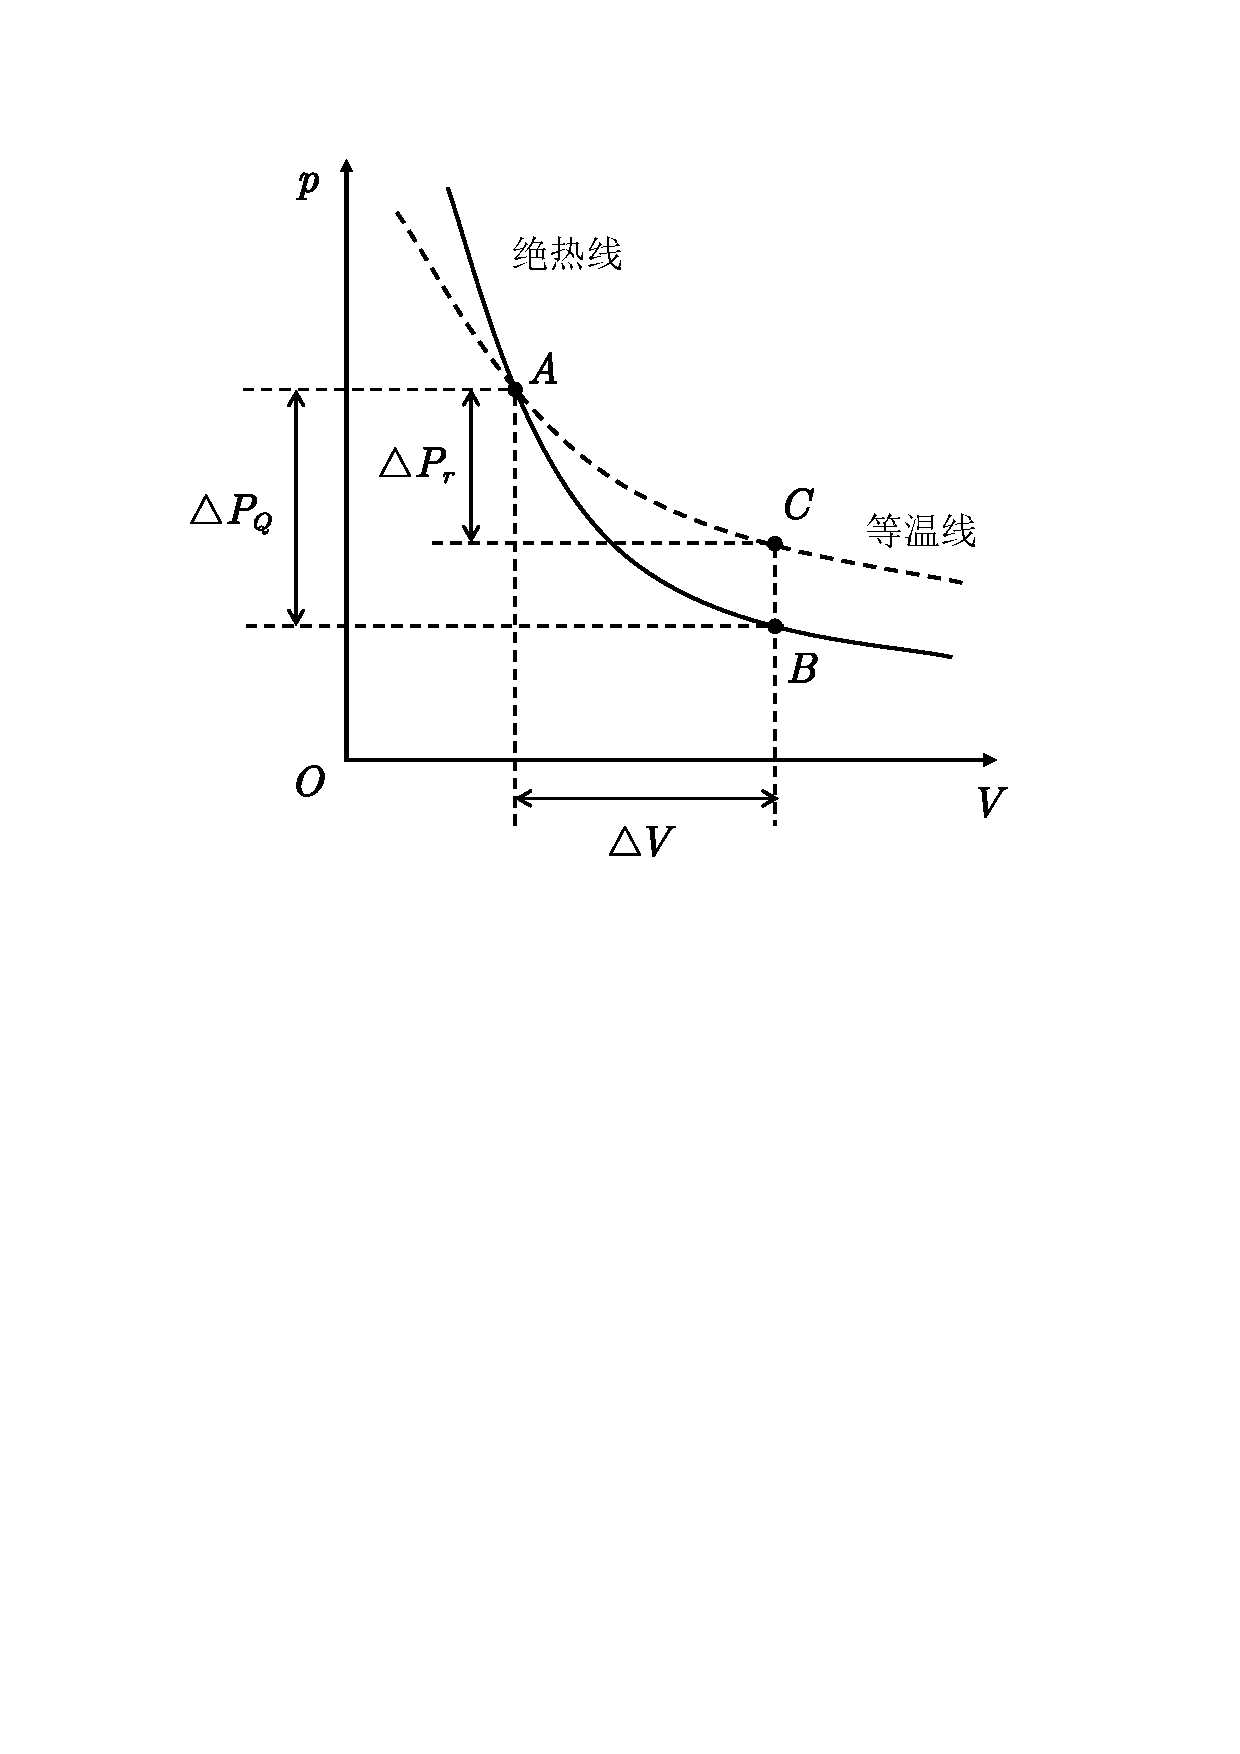
\includegraphics[scale=0.6]{Figures/pic1.pdf}  
\caption{绝热线与等温线的比较}
\label{fig1}
\end{figure}



\section{循环过程}
系统经历一个循环之后,其内能并没有改变,即$\bigtriangleup E=0$

在$p-V$图中,顺时针方向进行的为正循环,即热机;逆时针方向进行的为逆循环,即制冷机

\textbf{正循环与热机:}
\begin{figure}[H]

    \centering
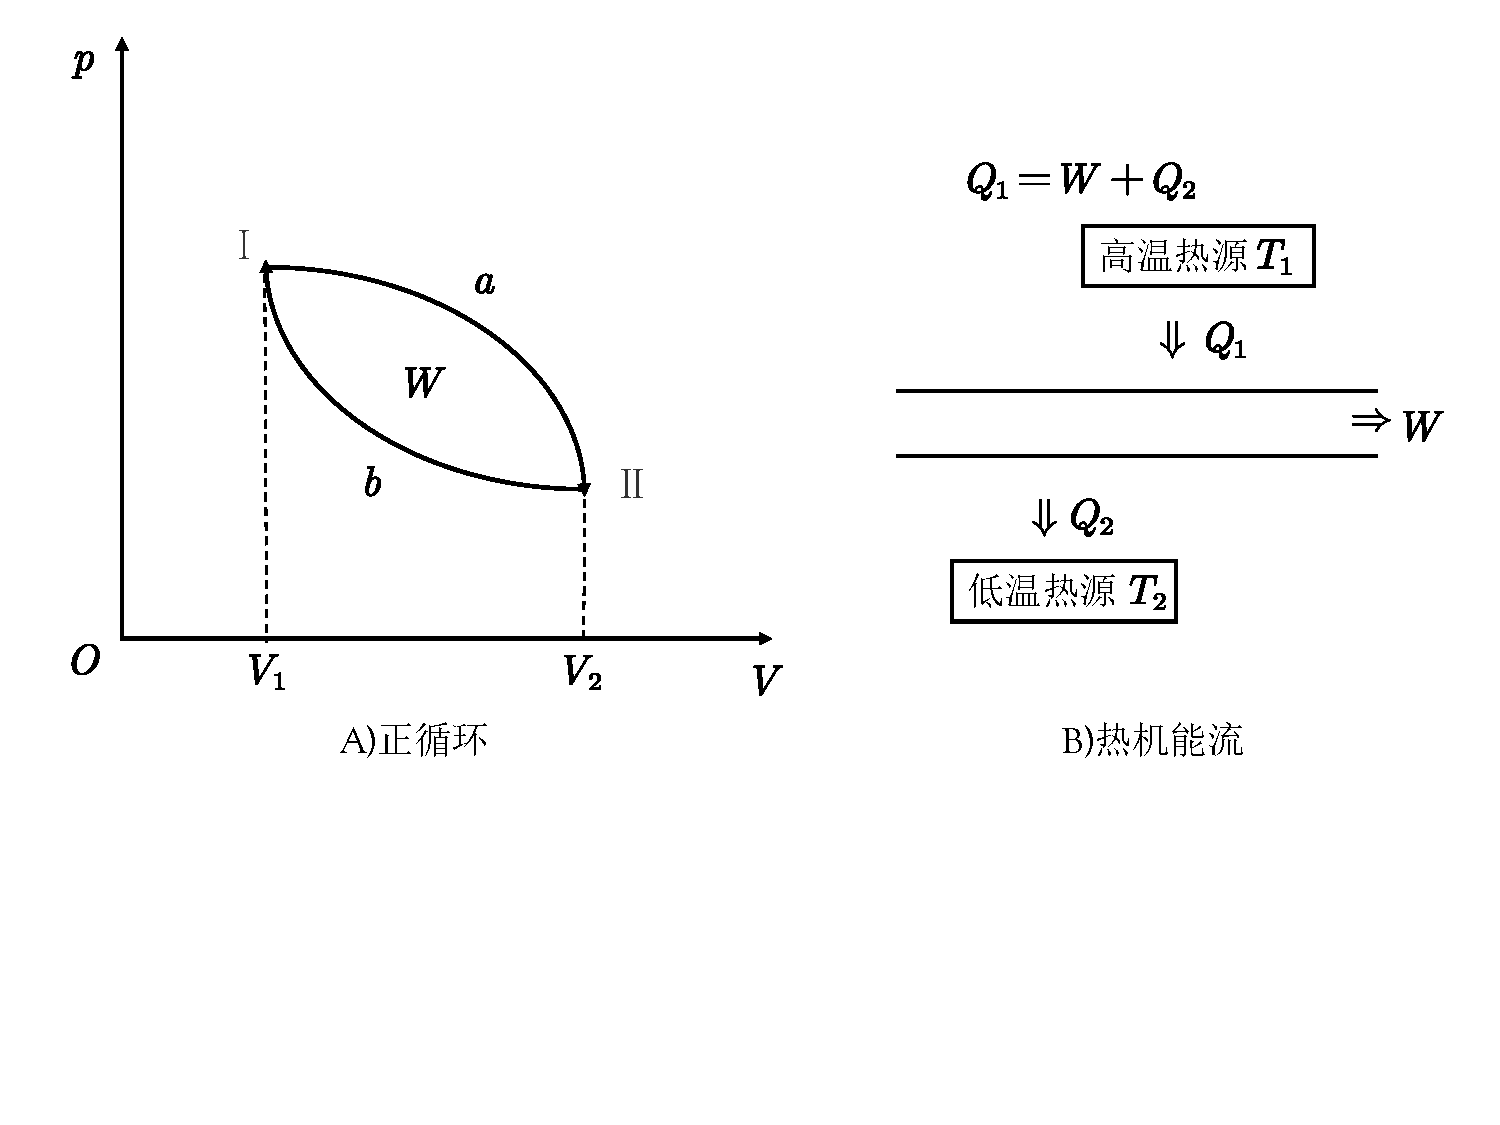
\includegraphics[scale=0.6]{Figures/pic2.pdf}  
\caption{正循环与热机能流图}
\label{fig2}
   
\end{figure}


\textbf{热机效率:}$\eta=\displaystyle\frac{W}{Q_1}=\frac{Q_1-Q_2}{Q_1}=1-\frac{Q_2}{Q_1}$


\textbf{逆循环与制冷机:}

\begin{figure}[H]

    \centering
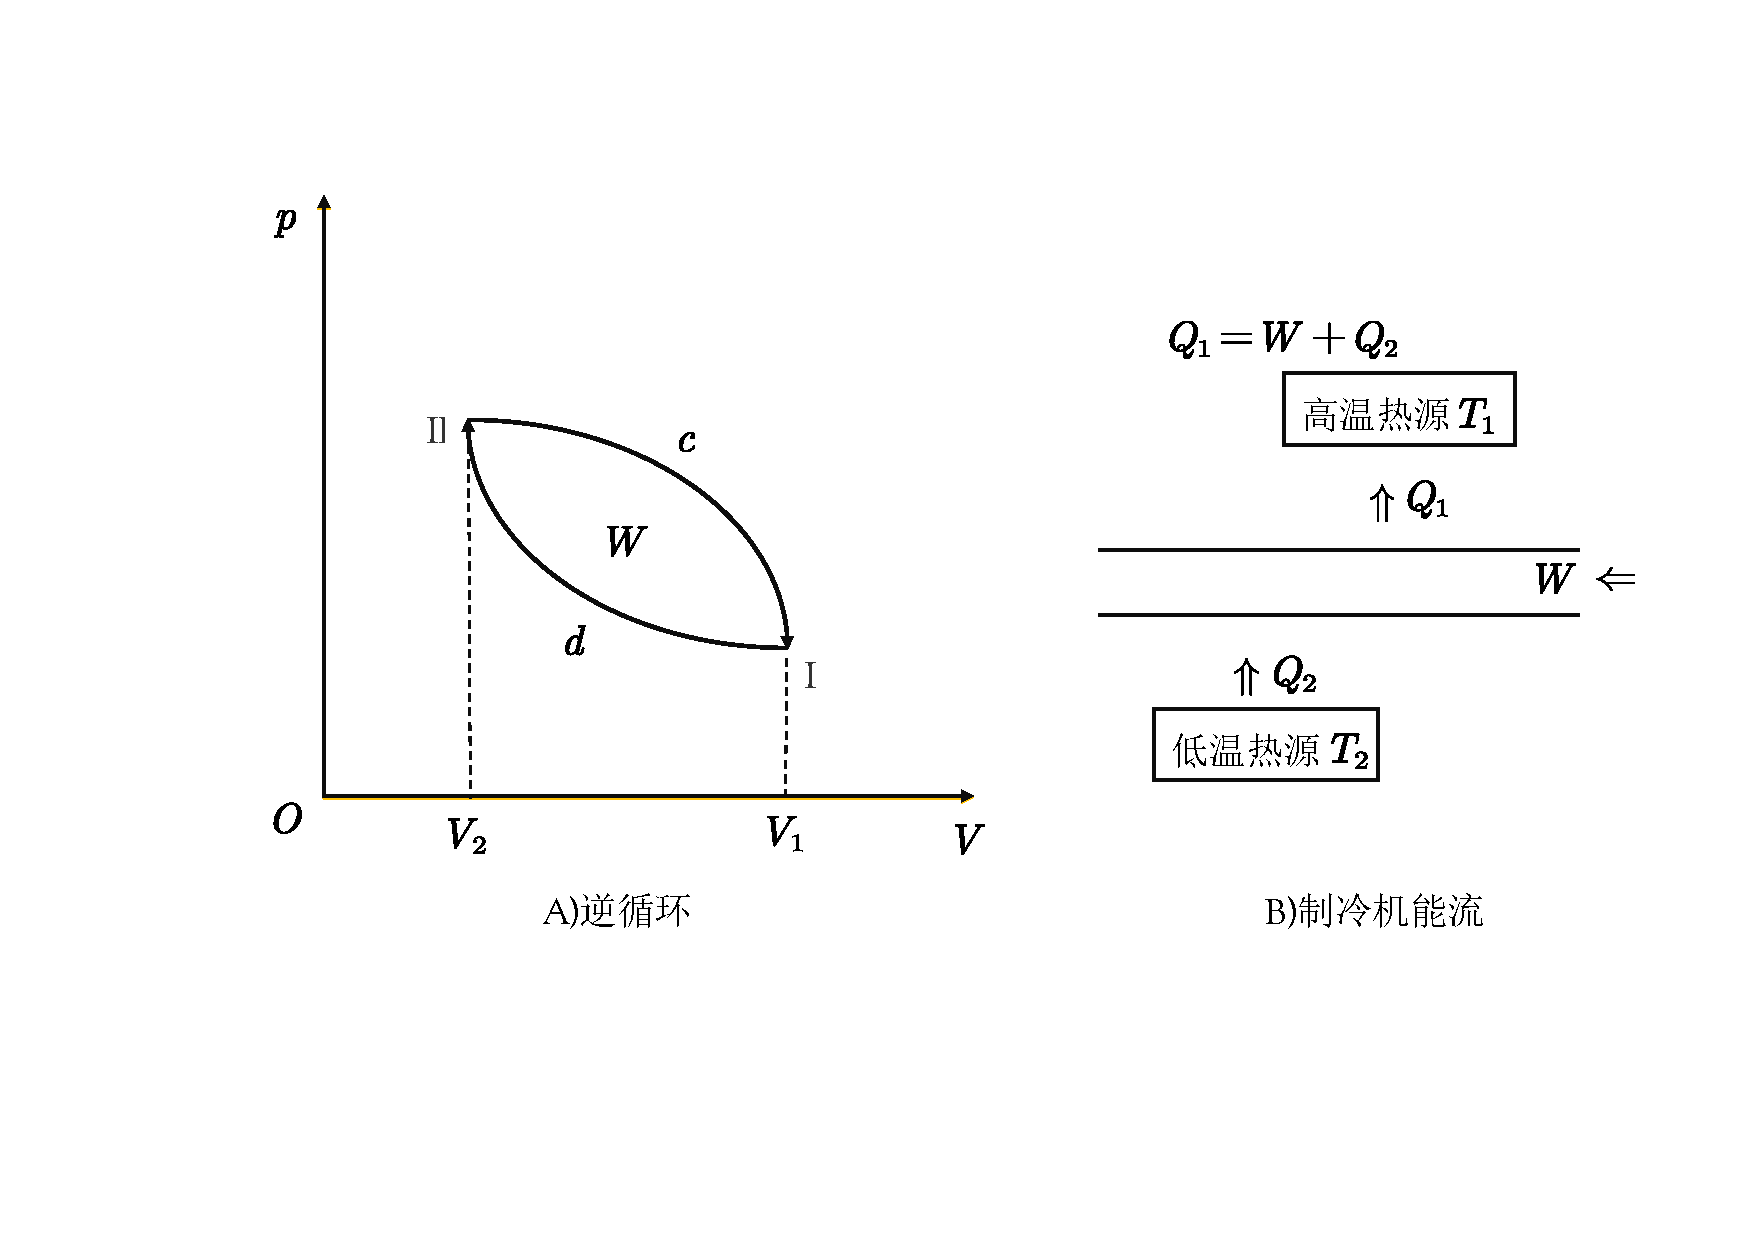
\includegraphics[scale=0.6]{Figures/pic3.pdf}  
\caption{逆循环与制冷机能流图}
\label{fig3}
\end{figure}



\textbf{制冷系数:}$e=\displaystyle \frac{Q_2}{W}=\frac{Q_2}{Q_1-Q_2}=\frac{T_2}{T_1-T_2}$


\textbf{卡诺循环:}

卡诺循环是由两个等温过程以及两个绝热过程组合而成,其工作过程如图8.4所示。其中$1\rightarrow2$为等温过程;$2\rightarrow3$为绝热过程;$3\rightarrow4$为等温过程;$4\rightarrow1$为绝热过程

\begin{figure}[H]

    \centering
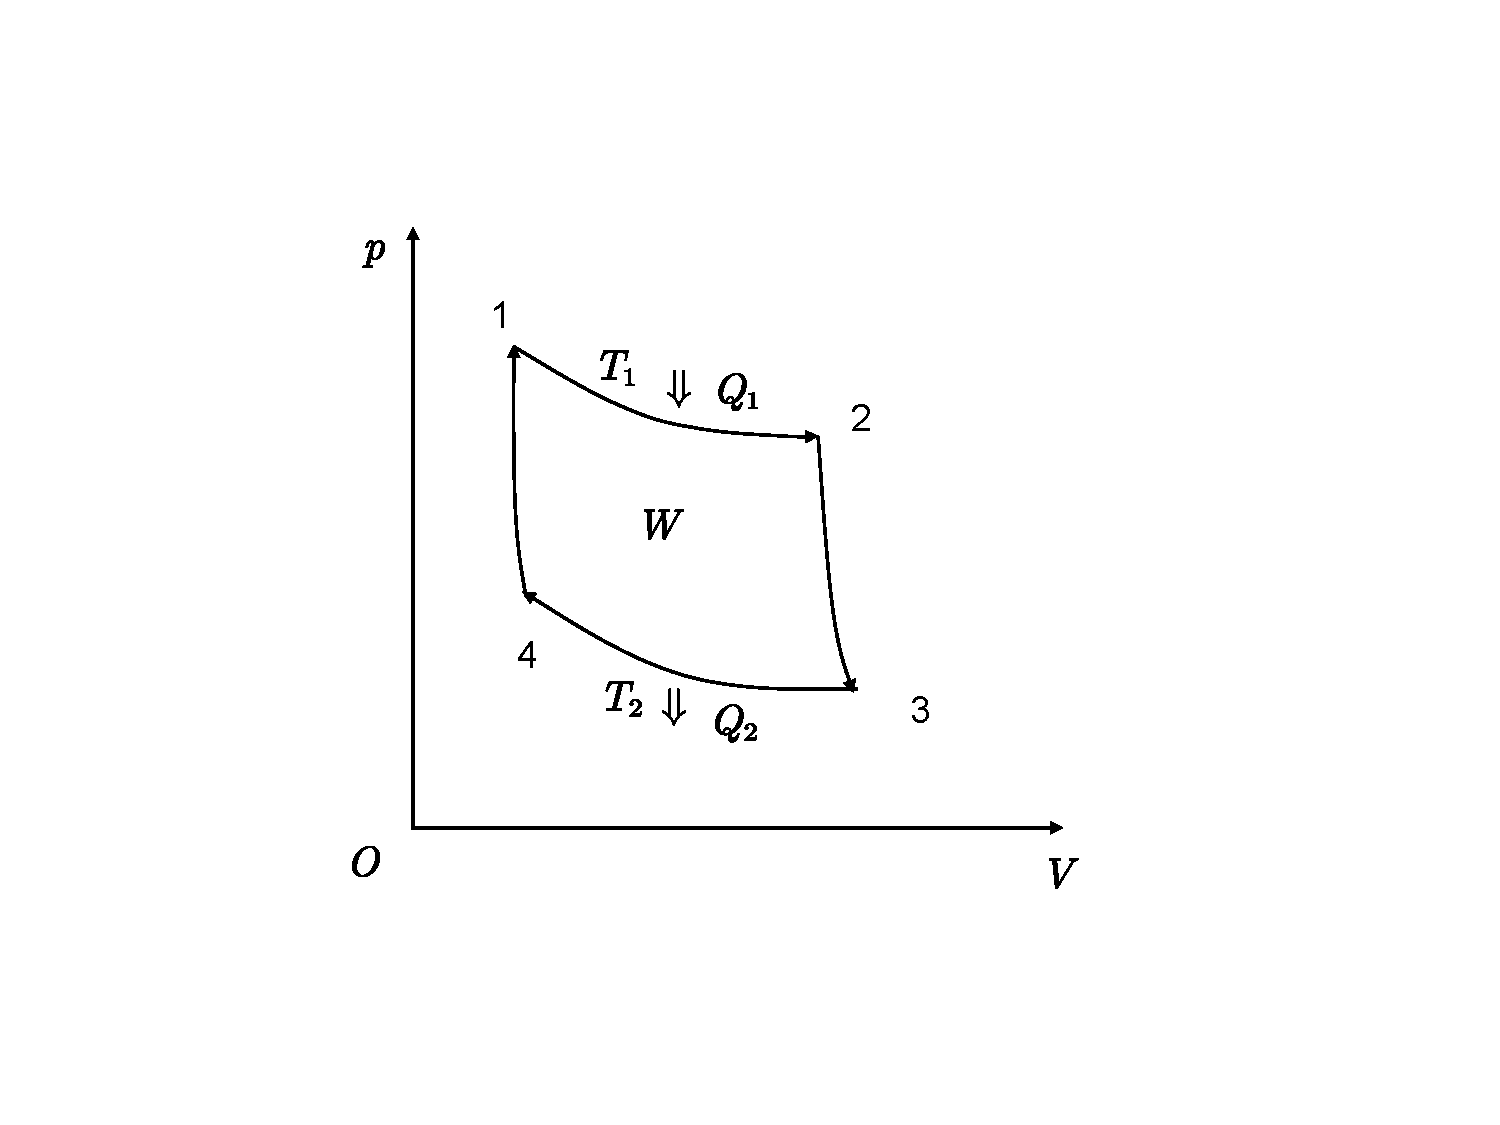
\includegraphics[scale=0.6]{Figures/pic4.pdf}  
\caption{卡诺循环}
\label{fig4}
\end{figure}


对于上图,有如下结论:
$$
\frac{Q_2}{Q_1}=\frac{T_2}{T_1}
$$
$$
\frac{V_2}{V_1}=\frac{V_3}{V_4}
$$
$$
\eta=1-\frac{Q_2}{Q_1}=1-\frac{T_2}{T_1}=\frac{T_1-T_2}{T_1}
$$


\textbf{卡诺逆循环:}
$$
e=\frac{Q_2}{W}=\frac{Q_2}{Q_1-Q_2}=\frac{T_2}{T_1-T_2}
$$

\textbf{若两个热源的$\bigtriangleup T$越大,卡诺循环的效率就越高}

\textbf{卡诺定理:}

\begin{itemize}
    \item 在相同的高温热源与低温热源之间工作的任意工质的可逆机,他们的效率均相等,即$\eta=1-\frac{T_2}{T_1}$

    \item 工作在相同的高温热源与低温热源之间的一切不可逆机的效率都不可能大于在同样两热源之间的可逆机的效率,即$\eta'\le 1-\frac{T_2}{T_1}$

\end{itemize}



\section{热力学第二定律}

\textbf{第二类永动机是不可能实现的}
\textbf{热力学第二定律的两种表述:}

\begin{itemize}
    \item \textbf{开尔文表述:}不可能制造出这样一种循环工作的热机,它只从单一热源吸收热量来做功而不放出热量给其他物体,或者说不使外界发生任何变化
    \item \textbf{克劳修斯表述:}不可能把热量从低温物体自动向高温物体传递而不引起外界的变化
\end{itemize}

\textbf{热力学第二定律的统计意义:}在一个不受外界影响的孤立系统中发生的一切实际过程,都是从概率小(微观态数少)的宏观态向概率大(微观态数多)的宏观态进行。与之相反的过程,并非绝对不可能发生,只是由于概率极小,实际上是观察不到的。此外,其还表明了它的适用范围只能是由大量微观粒子组成的宏观系统,对于粒子数很少的系统则是没有意义的


\section{熵}
热力学第二定律还可表述为在孤立系统中所进行的自然过程总是沿着熵增大的方向进行,它是不可逆的。平衡态对应的是熵最大的状态。这种表述称为\textbf{熵增加原理},其表达式为

若孤立系统经历的是可逆过程,则意味着过程中任意两个状态的热力学概率都相等,因而熵保持不变,有          ,结合上述,有      ,它表明:\textbf{孤立系统内无论进行什么过程,系统的熵永不减少}


















\end{document}